\chapter{Contre réactivité et contrôle de réacteur}
\section{Contre de réactivité}
	\subsection{Opération et contrôle}
	\begin{wrapfigure}[10]{l}{6.5cm}
	\vspace{-5mm}
	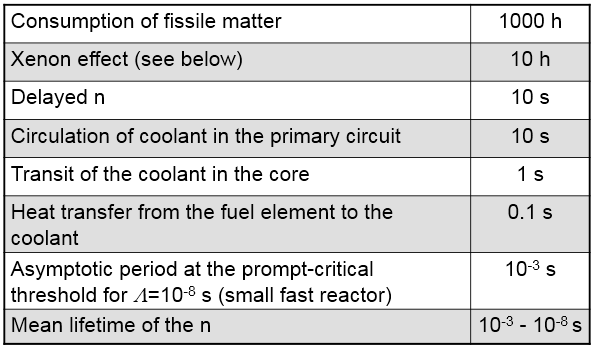
\includegraphics[scale=0.4]{ch6/image1.png}
	\captionof{figure}{Temps caractéristiques}
	\end{wrapfigure}
	La réactivité traduit la variation des paramètres du réacteur qui peuvent causer une perte du 
	cycle d'équilibre des neutrons et causer un transitoire : il est nécessaire de pouvoir contrôler 
	celui-ci dans toutes circonstances (arrêt, refroidissement rapide, nouveau combustible,\dots).\\
	
	On va donc introduire des marges de réactivités : le but est d'être capable d'introduire une 
	contre-réactivité en toutes circonstances. Ces marges de réactivités doivent être disponibles à 
	tout moment, de même magnitude et de signe opposé au changement de réactivité et dans un temps 
	caractéristique semblable à celui ou $\Delta \rho$ se produit.
	
	\subsection{Introduction à la théorie des perturbations}
	Il faut être capable d'estimer la réactivité dans un réacteur. Pour rappel, la réactivité est la 
	variation effective de $k_{eff}$
	\begin{equation}
	\rho  = 1 - \frac{1}{{{k_{eff}}}}
	\end{equation}	
	Il faudrait pouvoir l'estimer dans toutes les situations, mais c'est rarement possible :
	\begin{itemize}
	\item[$\bullet$] La réacteur du nucléaire n'est pas celle utilisée dans les calculs.
	\item[$\bullet$] Présence de détecteurs dans le cœur
	\item[$\bullet$] Consommation et production $f(t)$ des isotopes non-uniforme 		
	\end{itemize}
	Pour tout de même essayer d'estimer $\rho$ on va introduire une perturbation à partir d'un état
	de référence $K_0\varphi_0 = J_0\varphi_0$. On a donc comme état perturbé
	\begin{equation}
	K\varphi  = \frac{1}{{{k_{eff}}}}J\varphi \quad\Rightarrow\quad 
	\rho J\varphi  = (J - K)\varphi 
	\end{equation}
	
	\begin{wrapfigure}[6]{r}{5cm}
	\vspace{-5mm}
	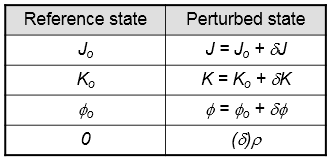
\includegraphics[scale=0.6]{ch6/image2.png}
	\captionof{figure}{ }
	\end{wrapfigure}	
	Considérons une fonction poids $\psi$ quelconque. La réactivité statique s'écrit (il s'agit d'un
	produit scalaire)
	\begin{equation}
	\rho  = \frac{{(\psi ,(J - K)\varphi )}}{{(\psi ,J\varphi )}}
	\end{equation}
	Introduisons un état de référence (désigné par un zéro) que l'on vient perturbé par une 
	perturbation $\delta$. En développant au premier ordre\footnote{Voir notes cours et TP8 de 
	TT.}
	\begin{equation}
	\rho (\psi ,{J_o}{\varphi _o}) = (\psi ,({J_o} - {K_o})\delta \varphi ) + (\psi ,(\delta J -
	\delta K){\varphi _o}) = ((J_o^* - K_o^*)\psi ,\delta \varphi ) + (\psi ,(\delta J - \delta K)
	{\varphi _o})	
	\end{equation}
	Soit $\varphi_0^*$ la solution du problème de référence adjoint $K_o^*\varphi _o^* = J_o^*\varphi
	 _o^*$. Si $\psi=\varphi_0^*$, alors 
	 \begin{equation}
	 \rho  = \frac{{(\varphi _o^*,(\delta J - \delta K){\varphi _o})}}{{(\varphi _o^*,{J_o}{\varphi
	  _o})}}
	 \end{equation}
	
	\subsection{Importance neutronique}
		\subsubsection{Sens physique du flux adjoint}
		Introduisions un neutron à un point $\bar r$ avec une vitesse $v\bar\Omega$ dans un 
		réacteur critique. Si celui-ci est placé en un point extérieur de la surface extérieure du
		réacteur (convexe) avec une direction de propagation sortante, il ne se passera rien
		\footnote{Il s'agit d'un problème qui aurait comme condition aux limites une quantité 
		pour les directions sortantes nulles. Dans le problème "de base", c'était nulle pour 
		entrante. Il s'agit d'une situation inverse, adjointe comme nous allons le voir.}. Si par
		contre on le place en plein milieu il aura plus d'impact : il peut jouer le rôle de 
		neutron secondaire et augmenter le flux mais à quel point ? Considérons le taux de 
		réaction\footnote{Expression obtenue au chapitre 2.} écrit à l'aide de la fonctionnelle 
		densité d'entrée \textit{f}
		\begin{equation}
		R = \int {  f(P)\psi (P)dP} 
		\end{equation}
		Avec (voir chapitre 2)\\
		
		\cadre{\begin{equation}
		\begin{array}{ll}
		\psi (P) &\DS= \int    Q(P')T(P' \to P)dP' + \int   \int\limits_{}    \psi (P)C(P \to P')T(P'
		\to	 P)dP'dP \\
		&\DS\equiv I(P) + \int    \psi (P')K(P' \to P)dP'
		\end{array}
		\end{equation}}\ \\
		
		Si au point $P$ le neutron subit une interaction, il y aura une contribution $f$ à ce point 
		$P$ qui doit être rajouté dans l'intégrale (pondère la densité d'entrée dans l'estimation du
		taux de réaction). Le neutron qui subit l'interaction n'est pas forcément capturé et peut 
		avoir une vie au delà de ça. S'il sort de l'interaction il est susceptible d'avoir un libre
		parcours moyen menant à une interaction ultérieure et contribué en une quantité $f$ du 
		point où il aboutit. \\

		On peut ainsi voir cette expression comme un terme source additionné à tout ce qui s'est passé
		\textbf{antérieurement} (tout ce qui vient des collisions et interactions au préalable qui 
		contribuent à ce qu'il y ai une densité d'entrée au point $P$). Nous avons en quelque sorte 
		"reversé" le problème (en regardant "précédemment") : il s'agit du problème adjoint qui est 
		plus facile à traiter que sa formulation avec Boltzmann.\\
		
		Le terme $H(P)$ donne l'importance d'un neutron entrant en collision au point $P$ pour le 
		taux de réaction $R$. Les contributions directes dues aux collisions au point $P$ valent 
		$f(P)$ et les contributions attendes pour les prochaines collisions 
		$\int    K(P \to P')H(P')dP'$.\\
		
		On peut alors définir l'\textit{équation adjointe} : $H(p)\equiv \psi^*(P)$ :\\
		
		\cadre{\begin{equation}
		\psi *(P) = f(P) + \int    K(P \to P')\psi *(P')dP'
		\end{equation}}\ \\
		
		Avec cette formulation adjointe, $f\psi$ peut s'exprimer en fonction du flux adjoint. Que 
		vaut alors l'expression du taux de réaction basé sur l'importance ? C'est le cas ou $n$ 
		neutrons sont émis par la source, puis transporté à la première collision\\
		
		\cadre{\begin{equation}
		R = \int {  f(P)\psi (P)dP}  = \int    I(P)\psi *(P)dP
		\end{equation}}\ \\
		
		On retrouve le produit de l'importance\footnote{On se souvient que son rôle est $\pm$ 
		important en fonction d'où il est place} d'un neutron au point $P$ pondéré par la 
		quantité de neutrons qui vont rentrer dans une première collision en ce point $P$.\footnote{
		Une bonne interprétation physique est disponible ici : \url{https://www.physicsforums.com/
		threads/
		what-exactly-is-an-adjoint-flux.414476/} ; "\textit{An adjoint calculation is basically a
		backwards calculation. Instead of starting with a neutron and calculating where it goes, you
		start with a fission event and calculate where the neutron that caused it could have come
		from. Adjoint flux is basically an importance factor for neutrons, and it's useful for
		radiation shielding and criticality analysis.}".}
		
		\subsubsection{Forme différentielle du problème de transport adjoint}
		Définissions nos deux opérateurs de création et destructions adjoints
		\begin{equation}
		\left\{\begin{array}{ll}
		{J^*} \bullet  &\DS= \frac{{\nu {\Sigma _f}(\bar r,v)}}{{4\pi }}\int_o^\infty     \int
		\limits_{4\pi }    \chi (v') \bullet dv'd\bar \Omega '\\
		{K^*} \bullet &\DS=  - \bar \Omega .\bar \nabla  \bullet  + {\Sigma _t}(\bar r,v) \bullet  -
		\int_o^\infty    \int\limits_{4\pi }   {\Sigma _s}(\bar r,v,\bar \Omega  \to v',\bar \Omega ')
		\bullet dv'd\bar \Omega '
		\end{array}\right.
		\end{equation}
		On utilisera alors les CL adjointe pour un réacteur dans le vide : la contribution des 
		neutrons sortant le long de la frontière est nulle
		\begin{equation}
		\forall {\bar r_s} \in \Gamma \;,\quad {\varphi ^*}({\bar r_s},v,\bar \Omega ) = 0\;\;if\;\;
		\bar n.\bar \Omega  > 0
		\end{equation}
		Dans le cas mono-cinétique, si $\varphi(\bar r, \bar \Omega)$ est la solution du problème 
		direct d'un réacteur de volume $V$ aux CL dans le vide, alors $\varphi(\bar r, -\bar \Omega)$
		est la solution du problème adjoint avec les CL adjointe dans le vide.
		
		\subsubsection{Problème de diffusion adjoint}
		Nos opérateurs adjoints sont
		\begin{equation}
		\left\{\begin{array}{ll}
		{J^*} \bullet  &\DS= \frac{{\nu {\Sigma _f}(\bar r,v)}}{{4\pi }}\int_o^\infty   \chi (v')
		\bullet dv'\\
		{K^*} \bullet  &\DS=  - \bar \nabla D(\bar r,v)\bar \nabla  \bullet  + {\Sigma _t}(\bar r,v)
		\bullet  - \int_o^\infty    {\Sigma _s}(\bar r,v \to v') \bullet dv'
		\end{array}\right.
		\end{equation}
		avec les CL extrapolée. Dans ce cas, le flux est auto-adjoint\footnote{Pourquoi?} : $\varphi
		\equiv\varphi^*$. Comme ces flux sont semblables les calculs en sont grandement 
		simplifiés\footnote{Voir trop\dots Ça sort d'où?} :
		\begin{equation}
		\rho  = \frac{{\int\limits_V    (\nu \delta {\Sigma _f}(\bar r) - \delta {\Sigma _a}(\bar r))
		{\varphi ^2}(\bar r)d\bar r}}{{\int\limits_V    \nu {\Sigma _f}(\bar r){\varphi ^2}(\bar r)d
		\bar r}}
		\end{equation}
		Ici, la variation de $\Sigma$ est pondérée par le flux au carré.
	
	
\section{Coefficient de réactivité}
	\subsection{Définition}
	Les variations de réactivité sont calculables par la théorie des perturbations, mais comment 
	retrouver les causes des variations de $J$ et $K$ ? Deux grandes causes
	\begin{enumerate}
	\item Modification de la densité en isotope
		\begin{itemize}
		\item[$\bullet$] Dilatation à cause d'une augmentation de la température
		\item[$\bullet$] Production et destruction d'isotopes
		\item[$\bullet$] Taux de vie (BWR mainly)
		\item[$\bullet$] Éjection de matière hors du primaire
		\end{itemize}
	\item Modification des sections efficaces microscopiques
		\begin{itemize}
		\item[$\bullet$] Effet Doppler (voir chapitre 8)
		\end{itemize}		
	\end{enumerate}
	Il y a également des effets causé par la variation de puissance, du carburant ou de la température
	du modérateur.
	
		\subsubsection{Variation $\delta T_c$ de la température du carburant}
		La section efficace se voit diminuée par augmentation de la température (moins de cible 
		lorsque la température augmente) mais positive dans le cas de Doppler
		\begin{equation}
		\delta \Sigma (\bar r) = \left(\underbrace{\frac{{\partial {N_U}(\bar r)}}{{\partial {T_c}}}}
		_{<0\text{ (dilatation)}}\sigma (\bar r) + {N_U}(\bar r)\underbrace{\frac{{\partial \sigma
		 (\bar r)}}	{{\partial {T_c}}}}_{>0\text{ (Doppler)}}	\right)\delta {T_c}(\bar r)
		\end{equation}
		Pour le modèle de la diffusion à une vitesse, Doppler est prédominant
		\begin{equation}
		\rho  = \frac{{\int\limits_V    (\nu {\Sigma _f}(\bar r)\frac{{\partial \ln {\sigma _f}}}
		{{\partial {T_c}}} - {\Sigma _a}(\bar r)\frac{{\partial \ln {\sigma _a}(\bar r)}}{{\partial
		 {T_c}}})\delta {T_c}(\bar r){\varphi ^2}(\bar r)d\bar r}}{{\int\limits_V  \nu {\Sigma _f}
		 (\bar r){\varphi ^2}(\bar r)d\bar r}}
		\end{equation}
		Supposons que $T_c(\bar r) = \theta_c(\bar r)$ avec $\theta_c$ la température moyenne et
		$f(\bar r)$ la distribution spatiale de $T_c$. \textbf{Si} une perturbation 
		$\delta T_c$ affecte seulement $\theta_c$ 
		\begin{equation}
		\frac{{\partial \rho }}{{\partial {\theta _c}}} = \frac{{\int\limits_V    (\nu {\Sigma _f}
		(\bar r)\frac{{\partial \ln {\sigma _f}(\bar r)}}{{\partial {T_c}}} - {\Sigma _a}(\bar r)
		\frac{{\partial \ln {\sigma _a}(\bar r)}}{{\partial {T_c}}})f(\bar r){\varphi ^2}(\bar r)d\bar
		 r}}{{\int\limits_V   \nu {\Sigma _f}(\bar r){\varphi ^2}(\bar r)d\bar r}}
		\end{equation}
		On appelle alors $\frac{{\partial \rho }}{{\partial {\theta _c}}}$ le coefficient de 
		réactivité. De façon plus générale : $N$ paramètres $\alpha_i$ indépendants
		\begin{equation}
		\delta \rho  = \sum\limits_i    \frac{{\partial \rho }}{{\partial {\alpha _i}}}\delta {\alpha
		 _i}
		\end{equation}
		Des exemples sont donnés au slide 11.
		
\section{Contrôle de réactivité à long terme}		
	\subsection{Contexte}
	\begin{wrapfigure}[7]{l}{6.5cm}
	\vspace{-5mm}
	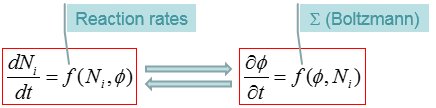
\includegraphics[scale=0.54]{ch6/image3.png}
	\captionof{figure}{ }
	\end{wrapfigure}	
	Jusqu'ici nous avons considérer les problèmes temporels (chapitre 5) sur des échelles de temps
	concernant les neutrons prompts et retardés mais il existe des effets à plus long terme : 
	consommation de carburant, décroissance des produits de fissions, \dots \\
	
	On parle d'\textbf{interactions} lorsque la consommation/production d'un matériau dépend du flux,
	qui dépend à son tour de la composition des matériau dans le réacteur (voir figure ci-dessus).\\
	
	Les échelles de temps sont susceptibles d'être différentes cependant, on traite généralement le 
	problème de la sorte
	\begin{enumerate}
	\item On calcule le flux en supposant $N_i$ constant à chaque intervalle de temps $\Delta t$ de 
	\textit{l'historique d'irradiation} du carburant (du début du cycle (BOC) jusqu'à la fin (EOC))
	(autrement dit, on mesure l'épuisement de la matière fissile).
	\begin{equation}
	\varphi ({T_{BOC}} + \Delta t) = f({N_i}({T_{BOC}}))
	\end{equation}
	\item On calcule l'évolution de $N_i$ à la fin de chaque pas de temps en considérant $\varphi$ 
	constant. En gros, sur la mise à jour de $N_i$ on va reconsidérer l'équation de Boltzmann avec
	une mise à jour du flux comme si tous ces $N_i$ avaient été constant jusque-là.
	\begin{equation}
	\frac{{d{N_i}(t)}}{{dt}} = f({N_i},\varphi ({T_{BOC}} + \Delta t))
	\end{equation}
	A la grosse louche, il s'agit d'un Euler explicite.
	\end{enumerate}
	\begin{center}
	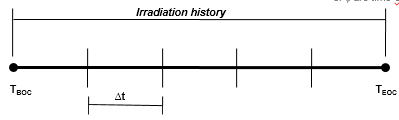
\includegraphics[scale=0.85]{ch6/image4.png}
	\captionof{figure}{Au début le combustible est frais et à la fin il ne reste plus rien : on 
	divise en intervalle $\Delta t$ pour voir les transitions.}
	\end{center}
	Ceci justifie les calculs de Burnup.

	\subsection{Évolution de la concentration en isotope}
		\subsubsection{Bilan des sources pour un isotope $i$}
		L'expression de l'évolution en isotope est donné par des équations super qui portent alors un 
		nom de super-héros : \textbf{équations de Bateman}\\
		
		\cadre{\begin{equation}
		\begin{array}{ll}
		\DS \frac{{d{N_i}}}{{dt}} = \sum\limits_j   &\DS\overbrace{ {\gamma _{ji}} \int    {N_j}{\sigma
		 _{f,j}}(v)	\varphi (v)dv}^{1} + \overbrace{\int {  {N_{i - 1}}{\sigma _{c,i - 1}}} (v)\varphi
		  (v)dv}^{2} + \overbrace{\sum\limits_j  	{\lambda _{j \to i}}{N_j}}^{3}\\
		&\DS - \underbrace{\left(\sum\limits_j   {\lambda _{i \to j}}\right){N_i}}_{4} - 
		\underbrace{{N_i}\int    {\sigma _{a,i}}(v)\varphi		(v)dv}_{5}
		\end{array}
		\end{equation}}\ \\
		
		Intéressons-nous d'abord aux sources positives
		\begin{enumerate}
		\item \textit{L'isotope $i$ vient de la fission d'un fragment}. Soit $\gamma_{ji}$ la fraction
		 des 
		fissions lié à l'isotope fissile $j$ donnant l'isotope $i$. L'intégrale donne le taux 
		de fission habituel associé à un isotope fissile $j$. On multiplie ensuite cette intégrale 
		par $\gamma_{ji}$ pour avoir la fraction des isotopes $i$ créé à partir des isotopes $j$.
		\item \textit{L'isotope $i$ résulte de la capture d'un neutron par un isotope $ i-1$.} La 
		capture d'un neutron peut contribuer à une augmentation de la quantité d'isotope présent dans 
		le réacteur (matériau fertile qui devient fissile en capturant un neutron).
		\item \textit{Décroissance radioactive des isotopes parents}. 
		\end{enumerate}
		Ces termes la ne sont pas forcément présents en même temps, mais l'un d'eux doit forcément
		être présent.\\
		
		Regardons maintenant les sources négatives
		\begin{itemize}
		\item[4.] \textit{L'isotope $i$ absorbe (capture et fission) un neutron}. En effet, on peut 
		avoir une certaine quantité de l'isotope $i$ qui provoque de l'absorption : cause de la 
		capture ou de la fission, mais dans les deux cas on ne retrouve plus l'isotope $i$ initial.
		\item[5.] \textit{Décroissance radioactive en isotope fille}.
		\end{itemize}
		Nous avons bien recensé toutes les contributions possibles.
		
\section{Effet du xénon}
	\subsection{Empoisonnement au xénon}
	La section efficace différentielle d'absorption $\sigma_a$ du $Xe^{235}$ aux énergies thermiques
	est de 2.7$\cdot10^6$ en 2200 ms$^{-1}$, elle joue donc un rôle important dans les produits de 
	fissions car elle va capturer une part importante des neutrons du réacteur. Sa production vient de
	la réaction suivante
	\begin{equation}
	Te^{135} \overset{\underset{\Longrightarrow}{\text{<0.5'}}}{\beta^-} I^{135} 
	\overset{\underset{\Longrightarrow}{\text{6.7h}}}{\beta^-} Xe^{135} 
	\overset{\underset{\Longrightarrow}{\text{9.2h}}}{\beta^-} Cs^{135} 
	\overset{\underset{\Longrightarrow}{2.6\cdot 10^6\text{ans}}}{\beta^-}\quad \text{(stable)}	
	\end{equation}
	La production du xénon vient de la désintégration radioactive $\beta^-$ de l'iode, un autre 
	produit de fission. Comme la production (par désintégration) du tellurium est très rapide, on 
	considèrera directement l'iode. En négligeant l'absorption de l'iode 135, on peut 
	écrire\footnote{$\lambda$ ? }
	\begin{equation}
	\left\{\begin{array}{ll}
	\dfrac{{dI}}{{dt}} &\DS= {\gamma _I}{\Sigma _f}\varphi  - {\lambda _I}I\vspace{2mm}\\
	\dfrac{{dX}}{{dt}} &\DS= {\gamma _X}{\Sigma _f}\varphi  + {\lambda _I}I - ({\lambda _X} + {\sigma
	 _{aX}}\varphi )X
	\end{array}\right.
	\end{equation}	
	où $X, I$ sont les densités atomiques en $Xe^{135}$ et $I^{135}$. La première relation vient 
	des équations de Bateman. Le premier terme de droite de la seconde équation est lié au courant 
	et le second au flux précédent. Ces deux éléments positifs (de source) correspondent à deux 
	situations temporelles transitoires.\\
	
	A flux constant, les solutions stationnaires sont données par
	\begin{equation}
	{I_\infty } = {\gamma _I}\frac{{{\Sigma _f}\varphi }}{{{\lambda _I}}},\qquad\qquad\qquad
	{X_\infty } = \frac{{({\gamma _I} + {\gamma _X}){\Sigma _f}\varphi }}{{{\lambda _X} + {\sigma
	 _{aX}}\varphi }}
	\end{equation}
	La saturation du Xe est obtenue pour\footnote{Justification de cette expression?}
	\begin{equation}
	\varphi  >  > \frac{{{\lambda _X}}}{{{\sigma _{aX}}}} \approx 0.775\,\,{10^{13}}n\;c{m^{ - 2}}{s^{
	 - 1}}
	\end{equation}
	On en tire alors la valeur maximale de la concentration en xénon en régime stationnaire à flux
	constant
	\begin{equation}
	{X_{\infty ,\max }} = \frac{{({\gamma _I} + {\gamma _X}){\Sigma _f}}}{{{\sigma _{aX}}}}
	\end{equation}
	
	
	Soit
	\begin{equation}
	\frac{{\varphi {\sigma _{aX}}{X_\infty }}}{{\varphi {\Sigma _f}}} = \frac{{({\gamma _I} + {\gamma
	 _X}){\sigma _{aX}}\varphi }}{{{\lambda _X} + {\sigma _{aX}}\varphi }}
	\end{equation}
	le rapport entre le nombre de neutrons absorbés par le xénon sur le nombre de neutrons de 
	fissions. On peut en tirer la réactivité (à un groupe)
	\begin{equation}
	\delta \rho  = \frac{{ - \int\limits_V   \frac{{({\gamma _I} + {\gamma _X}){\sigma _{aX}}{\Sigma
	 _f}\varphi (\bar r)}}{{{\lambda _X} + {\sigma _{aX}}\varphi (\bar r)}}{\varphi ^2}(\bar r)d\bar
	  r}}{{\int\limits_V    \nu {\Sigma _f}{\varphi ^2}(\bar r)d\bar r}}
	 - \frac{{({\gamma _I} + {\gamma _X})}}{\nu } =  - 0.027
	\end{equation}
	Cette réactivité négative est assez importante si l'on se souvient que le seuil prompt-critique
	vaut 1\$ ce qui correspond à 0.68\% : il faut prendre en compte cette chute car il y a une 
	possibilité d'arrêter le réacteur !
	
		\subsubsection{Arrêt du réacteur en régime asymptotique}
		Le réacteur étant à l'arrêt, les termes liés à la production d'isotopes disparaissent
		\begin{equation}
		\left\{\begin{array}{ll}
		\dfrac{{dI}}{{dt}} &= \DS - {\lambda _I}I\\
		\dfrac{{dX}}{{dt}} &\DS= {\lambda _I}I - {\lambda _X}X
		\end{array}\right.\qquad\Leftrightarrow\qquad\left\{\begin{array}{ll}
		I(\bar r,t) &\DS= {I_\infty }(\bar r){e^{ - {\lambda _I}t}}\\
		X(\bar r,t) &\DS= \frac{{({\gamma _I} + {\gamma _X}){\Sigma _f}{\varphi _o}}}{{{\lambda _X} +
		 {\sigma _{aX}}{\varphi _o}}}{e^{ - {\lambda _X}t}} + \frac{{{\gamma _I}{\Sigma _f}{\varphi
		  _o}}}{{{\lambda _I} - {\lambda _X}}}({e^{ - {\lambda _X}t}} - {e^{ - {\lambda _I}t}})
		\end{array}\right.
		\end{equation}
		On remarque que, à partir d'une certaine valeur du flux, la dérivée de la concentration en
		xénon est positive
		\begin{equation}
		{\left. {\frac{{dX}}{{dt}}} \right|_o} \ge 0\;\;iff\;\;\varphi  \ge \frac{{{\lambda _X}}
		}{{{\sigma _{aX}}}}\frac{{{\gamma _X}}}{{{\gamma _I}}} \approx 4\;{10^{11}}\;n\,c{m^{ - 2}}
		{s^{ - 1}}
		\end{equation}
		Lorsque l'on arrête le réacteur, non seulement le xénon était déjà gênant avant, mais en plus
		il augmente. La concentration en xénon augmente ainsi à cause des désintégrations de $I^{135}$ 
		sans destruction du flux neutronique (maximum après 11h) puis il décroit. Si le flux augmente
		depuis un régime stationnaire, la concentration en xénon va premièrement diminuer pour 
		ensuite augmenter\footnote{Un autre isotope (poison) a le même effet : Sm.}.
	
	\subsection{Oscillations dues aux xénon}
	Considérons un réacteur de grande taille telle que $R/L \gg 1$. Considérons deux régions 
	suffisamment distantes, toutes les deux critiques et qui peuvent être vue comme $\pm$ découplée
	\footnote{Il faudrait quelques explications sur le tableau slide 19, pas tout compris avec les
	différentes zones.}.
	\begin{enumerate}
	\item En $t=0$, le flux commence à diminuer.
	\item A court terme, la concentration en xénon commence à augmenter à cause des fissions d'une 
	dizaine d'heures plus tôt (la concentration en Xe dépend du flux des heures précédentes car c'est
	lui qui a généré l'iode). La réactivité est donc négative et il en résulte une autre diminution 
	du flux.
	\item A long terme, la concentration en Xe diminue (désintégration), la réactivité redevient 
	positive et le flux augmente.
	\end{enumerate}
	Il faut donc bien être conscient que les produits de fissions qui apparaissent ne sont pas 
	forcément inactifs sur le fonctionnement du réacteur.
	
	
	
\section{Moyens pour assurer le contrôle}
	\subsection{Moyens externes}
	Les barres de contrôles (isotope neutrophage) peuvent diminuer le flux mais il faut faire 
	attention à la position de celles-ci (la diminution du flux se fait dans leur voisinage). Avec 
	elles, on peut avoir une source de réactivité positive ou négative (et même prompt dans le 
	cas d'un scram). Il existe aussi les poisons chimiques comme l'acide borique qui permet d'agir
	plus uniformément.\\
	
	Il y a également les poisons consommables. Par un élan de flemme assez important, voici mes notes
	de cours non retravaillées : "\textit{Y’a aussi les poisons consommables. Quand on ferme le couvercle on le fait tourner non stop (on espère). Mais les concentrations varie : pour maintenir la criticité du début à la fin de cycle le réacteur au départ avec du combustible frais est fortement supercrituqe. Ca peut sembler bizarre car bcp de neutrons produits mais dont on consomme une partie par ce genre de poison dont la cencentration baisse progressivement on peut se retrovuer a un niveau $k_{eff}$ élevé au départ maisa vec la possibilité de pas etre hors ctrl dans le réacteur. 
}"
	


	
	
	
	\subsection{Évolution de la réactivité}
	
	
		
	
\iffalse
\fi	